%Kontext: Benutzerdokumentation Projekt CodeRed
%Changelog:
%Timestamp                      Name                      Äderungen und Begründung
%

%Dokumentklasse und einige globale Einstellungen
\documentclass[11pt,a4paper,titlepage,openright,multicol]{scrbook}

%Untersttzung für Zeichen außrhalb des ASCII-Zeichensatzes
\usepackage[utf8]{inputenc}
\usepackage{fontenc}

%Trennungsregeln
\usepackage[ngermanb]{babel}

\usepackage{multicol}

%zahlreiche Pakete und weitere Einstellungen
\usepackage{color}
\usepackage{fancyhdr}

%\usepackage[a4paper,left=3cm,right=1.5cm,headheight=1.5cm]{geometry}
\usepackage{ngerman}
\usepackage[pdftex]{graphicx}

\usepackage[pdftex, bookmarks,
		colorlinks=true,
		linkcolor=black,
		urlcolor=black,
		pdftitle={CodeRed Unterweisung},
		pdfauthor={Marco Benecke, Jan Neuser},
		pdfsubject={Eine Unterweisung in die Software CodeRed}
		pdfkeywords={ADA, Unterweisung, Codered, STSWeilburg}]{hyperref}


\usepackage{longtable}

%Erstellung einer Indexdatei
\usepackage{makeidx}

\usepackage{textcomp}
\usepackage{verbatim}

%Verwendung von Font Type 1 fr bessere Lesbarkeit im Acrobat Reader
\usepackage{pslatex}

%Gliederungstiefe, Makropaket und Einstellung fr das Inhaltsverzeichnis
\usepackage{minitoc}
\setcounter{secnumdepth}{3}
\setcounter{tocdepth}{2}

%Aufnahme der Verzeichnisse (Stichwortverzeichnis, Abbildungs- und Tabellenverzeichnis) ins Inhaltsverzeichnis
\usepackage{tocbibind}

\usepackage{nomencl}

\usepackage{listings}
%in der aktuellen Version des Styles fr listings haben sich einige �derungen ergeben, insbesondere wird label durch number ersetzt, das Stylefile wird nicht mehr ausgeliefert
%\lstset{captionpos=b, frame=trbl, frameround=ffff, labelstyle=\tiny, labelstep=5, firstlabel=1, labelsep=5pt}
%\lstset{captionpos=b, frame=trbl, frameround=ffff, numberstyle=\tiny, stepnumber=5, firstnumber=1, numbersep=5pt, aboveskip=10pt, belowskip=10pt}

% weitere Eigenschaften fr den Abstand des Listings
% aboveskip=10pt, belowskip=10pt

\usepackage{path}

% Das Paket parskip verhindert den Einzug am Anfang neuer Abs�ze und setzt einen sinnvollen Zeilenabstand zwischen den Abs�zen, wirkt sich darber hinaus auch Einrckungen in Aufz�lungen, Listen usw. aus.
\usepackage{parskip}

%sollte Fussnoten in Tabellen erm�lichen, berfordert aber Latex
%\usepackage{./texstyles/ftn}
%\ftn{tabular}

\makeatletter
%Breite fr die Seitennummerierung in Inhaltsverzeichnis
%Vermeidung des Fehlers Overfull \hbox
\renewcommand{\@pnumwidth}{2.5em}

%Abstand zwischen der Abschnittsnummer und der Kapitelberschrift im Inhaltsverzeichnis
\renewcommand*\l@section{\@dottedtocline{1}{1.0em}{2.3em}}
\renewcommand*\l@subsection{\@dottedtocline{2}{3.3em}{3.2em}}
\renewcommand*\l@subsubsection{\@dottedtocline{3}{6.5em}{4.1em}}
\renewcommand*\l@paragraph{\@dottedtocline{4}{9.5em}{5.0em}}
\renewcommand*\l@subparagraph{\@dottedtocline{5}{11.5em}{6.0em}}

%Kapitelnummerierung am Anfang jedes Buches, eingeleitet durch \part zurcksetzen
%Kompiliert jetzt zwar korrekt, verhindert aber ein vernnftiges Bookmarking durch das Paket hyperref
%\@addtoreset{chapter}{part}
\makeatother

%Seitennummerierung in arabischen Ziffern
%\pagenumbering{arabic}

\makeindex
\makeglossary

%Anfang des Dokuments
\begin{document}

%Einleitung mit eigenen Seitennummerierung
\frontmatter

%Hauptteil
\mainmatter

%Titelseite
%Kontext: Komplettes Handbuch für Codered
%Changelog:
%Timestamp			Name			Äderungen und Begründung
%

\begin{titlepage}

\title{- \textbf{CodeRed} -\\ 
\mbox{Das \textit{Trouble Ticket System}} \\
- der Staatliche Techniker Schule Weilburg  - \\
- Benutzerhandbuch -}
\author{Marco Benecke \and Jan Neuser}
\date{Ausgabe 0.1 vom \today}


\publishers{Staatliche Techniker Schule Weilburg}

\uppertitleback{

\textbf{Version:} \\
- Projekt Dokumentation \\
- CodeRed Server Administration \\
- \underline{CodeRed Benutzer Dokumentaion} \\
% use packages: array
\begin{tabular}{ll}
Thema: & CodeRed - Handbuch - Benutzer\\
Server & Version: CodeRed RC2 Version 0306 \\
Datum: &  10.04.06\\ 
Puplic Version: & CodeRed System RC2 \\  
\end{tabular}

\vspace{2cm}

\textbf{Autoren:} \\
Benecke, Marco erreichbar unter \textit{benecke@gmail.com} \\
Neuser, Jan mit \textit{jan@truematrix.de} \\

\vspace{1cm}

\textbf{Korrekturleser:} \\
 Cristine Holzhäuser \\
 Beate Neuser \\
 Anne Neuser \\
}

\lowertitleback{Dieses Buch unterliegt den Grundgedanken der GPL und wird ausschließich mit Hilfe des Satzsystems {\LaTeX} unter Linux geschrieben. Die Veröffentlichung erfolgt als plattformunabhägiges PDF. Vielen Dank.}

\maketitle

\end{titlepage}



%Inhaltsverzeichnis
\tableofcontents

\part{Einleitung}
\label{part:Einleitung}
\chapter{Die Idee}  % Kapitel % Steht dann über dem Text
\label{chapter:Die Idee}  % Steht als Text im Inhaltsverzeichnis
\index{Die Idee} % für das Stichwortverzeichnis

Die Staatliche Technikerschule Weilburg (STSW)
übernimmt seit Jahren verschiedene IT Projekte
von Firmen und Schulen im Rahmen der praktischen
Abschlussprüfungen der angehenden Techniker. \\
\\
Nun stellte sich heraus, dass mit der Zeit
Wartungsarbeiten an den Projekten anfallen oder
dass Defekte behoben werden müssen.
Die Schulen, die selbst keine Ressourcen für die
Problembehebung bündeln konnten, haben sich
wieder an die STSW gewannt, um Hilfe bei ihren
Problemen zu bekommen. \\
\\
Diese Probleme wurden an einen Lehrer weitergeleitet,
dieser löste diese entweder selbst oder
beauftragte einige Studierende mit der Lösung.
Schwierigkeiten bestanden darin, dass meist nur noch die
Dokumentation des Projektes zur Lösungshilfe bereit
steht. Alle Änderungen und evtl. schon vorhandene
gelöste Probleme sind nicht dokumentiert gewesen und gingen
somit immer mit dem Abschluss der Studierenden verloren.\\
\\
Die Lösung für diese vielen Probleme wurde unter dem Namen \textbf{CodeRed} 
entwickelt. Ca ein Jahr hat sich das Team gedanken über eine Lösung und 
deren umsetzung gedanken gemacht. CodeRed verwaltet zentral alle Probleme 
die bei den Klienten entstehen. Das System ist webbasierend und dadurch von jedem 
Anwender mit einem Internetzugang anwendbar. Serviceteams, Clienten, Kontakte oder auch Mentoren können über die Datenbankapplication schnell und einfach ihre Probleme oder Lösungen dokumentieren. \\
\\
Bei der Entwicklung wurde besonders darauf geachtet, die komplexen Abläufe die Auftreten können, klar und einfach zu halten. Niemand sollte eine gößere Einführung in die Software benötigen um sie Nutzen zu können. Deswegen wurde auf neue Technologien die unter dem Begriff Web2.0 in den Fachmedien bekannt geworden sind, großen Wert gelegt.\\
\\
Wir die Entwickler hoffen eine leistungfähige Lösung entwickelt zu haben, die von jedermann bedient werden kann.   

\chapter{Entwickler}  % Kapitel % Steht dann über dem Text
\label{chapter:Entwickler}  % Steht als Text im Inhaltsverzeichnis
\index{Entwickler} % für das Stichwortverzeichnis

Als Entwickeler von CoderRed möchten wir uns gerne hier kurz vorstellen, wir stehen allen die weitere Fragen zu diesem Projekt haben natürlich gerne zur Verfügung. \\
\\
Allgemein besteht das Entwickelerteam von CodeRed aus zwei Studierenden der Staatlichen Techniker Schule Weilburg. Wir haben im Jahr 2004 die Ausbildung zum Staatlichen Techniker der Informationstechnik, Schwerpunkt Computersystem und Netzwerktechnik begonnen und Sommer 2005 dieses Projekt übernommen. Für uns stand bei der Übernahme der Aufgabe vorallem eines im Vordergrung, wir wollen unbedingt etwas machen was wir noch nicht beherschen und wir viel Lernen könnten. So war die Entwicklung eines Webbasierenden Trouble Ticket System eine nahe zu ideale Aufgabe, auch wenn wir erst nicht wussten wie wir diese Aufgabe lösen sollten.   
\\
\\
Backend Entwickeler \\
\textbf{Marco Benecke}
\\
\begin{picture}(150,200)

\includegraphics{../bilder/marcob.jpg}
\end{picture}
\\
Marco Benecke \\
Bitzengarten 16 \\
35614 Asslar-Oberlemp \\
\\
\textbf{Konatkt} \\
\begin{itemize}
\item Mobil: 0175 - 74 10 565
\item E-Mail: benecke@gmail.com
\item JabberID: Risktaker@jabber.org 
\item Homepage: \href{http://www.bytes-delivery.de}{bytes-delivery.de}
\end{itemize}
\textbf{Werdegang} \\
\begin{itemize}
\item Realschulabschluss auf der Gesamtschule Asslar-Hermannstein
\item Ausbildung zum Energieelektroniker-Betriebstechnik bei der Buderus Guss GmbH in Wetzlar
\item 5./Technische Schule der Luftwaffe in Erndtebrück Staabsgebiet 6 – Netzbetreuer und Administrator
\item Weiterbildung zum Staatlich geprüften Techniker in Weilburg, Schwerpunkt: Computersystem und Netzwerktechnik	
\end{itemize}
FrontEnd Entwickeler \\
\textbf{Jan Neuser}
\\
\begin{picture}(150,200)

\includegraphics{../bilder/marcob.jpg}
\end{picture}
\\
Jan Neuser \\
Münchbornstr.4 \\
35753 Greifenstein Arborn \\
\\
\textbf{Konatkt} \\
\begin{itemize}
\item Mobil: 0177 - 60 39 783
\item E-Mail: jan@truematrix.de
\item JabberID: nean77@gmail.com 
\item Homepage: \href{http://www.truematrix.de}{truematrix.de}
\end{itemize}
\textbf{Werdegang} \\
\begin{itemize}
\item Realschulabschluss auf der Gesamtschule Driedorf
\item Ausbildung zum IT- Systemelektroniker in Sinn bei der Firma Dietermann \and Heuser GmbH  (Heute: Hees Bürowelt)
\item Stabskompanie Panzerbrigade 14, Stabsdienst - Truppenverwaltung
\item Weiterbildung zum Staatlich geprüften Techniker in Weilburg, Schwerpunkt: Computersystem und Netzwerktechnik	
\end{itemize}



\chapter{Lizenzen}  % Kapitel % Steht dann über dem Text
\label{chapter:Lizenzen}  % Steht als Text im Inhaltsverzeichnis
\index{Lizenzen} % für das Stichwortverzeichnis

\begin{figure}[h]
\begin{center}
   
\includegraphics[width=130pt]{../bilder/gnu-head-sm.jpg}
   \caption{GNU Projekt Logo}
   \label{GPL Lizenz}
\end{center}
\end{figure}
Das Projekt CodeRed unterliegt in seinen Grundzügen der \href{http://de.wikipedia.org/wiki/GPL}{GPL Lizenz} und wurde mit Hilfe von Freien Software Produkten und Entwicklungsumgebungen geschaffen.
\begin{figure}[h]
\begin{center}
   
\includegraphics[width=90pt]{../bilder/mysql.jpg}
   
\includegraphics[width=90pt]{../bilder/rails.png}
   
\includegraphics[width=90pt]{../bilder/debian.png}
   
\includegraphics[width=90pt]{../bilder/apache.png}
   \caption{GNU Projekt Logo}
   \label{GPL Lizenz}
\end{center}
\end{figure}
\chapter{Danksagung}  % Kapitel % Steht dann über dem Text
\label{chapter:Danksagung}  % Steht als Text im Inhaltsverzeichnis
\index{Danksagung} % für das Stichwortverzeichnis

Das Projekt CodeRed konnte nur durch die Unterstützung von vielen verschieden Personen und Freien Internet Diensten verwirklicht werden. So möchten wir uns bei allen Menschen und Institutionen für ihre Ideen, Kretik und ihr Lob bedanken. \\
Ein paar Vorbilder und Hilfen für die Umsetzung dieses Projektes waren: 
\\
\textbf{Dienste und Pattformen}
\begin{itemize}
\item \href{http://www.berlios.de}{BerliOS}, die jedem Entwickeler eine sehr gute freie Kommunikatiosplattform zur verfügung stellt,
\item \href{http://www.google.de}{Google}, mit ihren Entwicklungen wie Gmail waren sie ein sehr großes Vorbild in Sachen Anwenderfreundlichkeit. 
\item \href{http://rubyonrails.de}{ROR Entwickler Deutschland}, mit ihrer Hilfe über die Mailingliste haben sie uns über einige Fehler hinweggeholfen
\end{itemize}

\part{CodeRed -Allgemein}
\label{part:CodeRed -Allgemein}
\chapter{Was macht CodeRed?}  % Kapitel % Steht dann über dem Text
\label{chapter:Was macht CodeRed?}  % Steht als Text im Inhaltsverzeichnis
\index{Was macht CodeRed?} % für das Stichwortverzeichnis

Text was CodeRed überhaupt macht?!


urls bitte so:
\href{http://codered.berlios.de}{Codered Projektseite}


für consolen komandos:
\verb|kommando -option parameter|


\chapter{Wie funktioniert CodeRed?}  % Kapitel % Steht dann über dem Text
\label{chapter:Wie funktioniert CodeRed?}  % Steht als Text im Inhaltsverzeichnis
\index{Wie funktioniert CodeRed?} % für das Stichwortverzeichnis

CodeRed ist ein Webbasierendes Online Ticket System. Als dieses ist das System für jeden unter einer öffentlichen Subdomäne aus dem Internet erreichbar. \\
\\
Jeder der das System Nutzen will, muss sich an dem System als erstes Registrieren. Nach erfolgreicher Anmeldung, wird der neue User direkt in sein persönliches Profil weitergeleitet. Dort kann er seine Daten Ändern oder Ergänzen. Zusätzlich hat der User die Möglichkeit in seinem Profil ein Avatar einzurichten.\footnotemark[1] \\
\\
Der neu angelegte User ist per default erst mal im System deaktiviert, er besitzt also keine weiteren Rechte. Er kann sich nur in dem System Umschauen und sein eigenes Profil Anschauen und Ändern. Um produktiv in dem System zu werden muss der neue User von einem Mentoren in seine vorgesehene Position gehoben werden. Der Mentor stuft den User als Kontakt, Betreuer oder auch als Mentor ein. Der User bekommt per E-Mail eine Benachrichtigung über die Änderung und kann sich dann mit seinem neuen Nutzerstatus am System neu Einlogen.\\ 
\\
Je nach seinem Status kann der User dann in dem System arbeiten. Die einzelnen Aufgaben und Rechte werden auf dem folgeden Seiten ausführlich erläutert.


\footnote[1]{Ein Avatar ist eine künstliche Person oder ein grafischer Stellvertreter einer echten Person in der virtuellen Welt.Avatare werden beispielsweise in Form eines Bildes, Icons oder als 3D-Figur eines Menschen oder sonst irgend eines Wesens dargestellt.}  



\chapter{Wo und Wie?}  % Kapitel % Steht dann über dem Text
\label{chapter:Wo und Wie?}  % Steht als Text im Inhaltsverzeichnis
\index{Wo und Wie?} % für das Stichwortverzeichnis

CodeRed kann jeder Nutzen der sich am System angemeldet hat. Wer welche Position oder Aufgaben im System übernimmt entscheiden die schon vorhandenen Mentoren. Ein User von Außerhalb kann sich zwar am System registrieren, ohne weiteren Kontakt zu einem Mentoren bleibt sein Account aber deaktiviert.\\
\\
Das Projekt CodeRed ist unter:\\
\centerline{\href{http://help.stsweilburg.de}{\textbf{http://help.stsweilburg.de}}\\ \href{https://help.stsweilburg.de}{\textbf{https://help.stsweilburg.de}}} \\
erreichbar.\\
\\ 
Zum Schutz ihrer Daten empfehlen wir den Zugang über die Sichere SSL\footnote[1]{Transport Layer Security (TLS) oder Secure Sockets Layer (SSL) ist ein Verschlüsselungsprotokoll für Datenübertragungen im Internet. TLS 1.0 und 1.1 sind die standardisierten Weiterentwicklungen von SSL 3.0.} Verbindung.
\newpage
\begin{figure}[h]
\begin{center}
   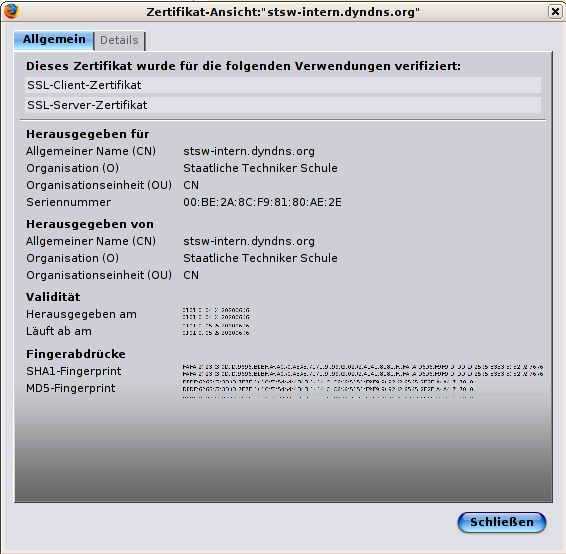
\includegraphics[width=370pt]{../bilder/certs2.png}
   \caption{Sichere SSL Verbindung}
   \label{Sichere SSL Verbindung}
\end{center}
\end{figure}
Für die Verschlüsselte Verbindung benutzt CodeRed ein Zertifikat mit einer 2048 Bit Verschlüsselung Da der Browser dieses Zertifikat nicht automatisch kennt, fragt der Browser den User ob das Zertifikat vertrauenswürdig ist. Um eine Verschlüsselte Verbindung aufzubauen muss hier das Zertifikat auf jedenfall angenommen werden. Ein Zertifikat das schon vom Browser als Sicher erkannt wird, kostet leider meist viel Geld. Für eine gesicherte Verbindung ist solch ein Zertifikat aber nicht nötig. 




\part{CodeRed -Arbeitsumgebung}
\label{part:Arbeitsumgebung}
\chapter{Erste Schritte}  % Kapitel % Steht dann über dem Text
\label{chapter:Erste Schritte}  % Steht als Text im Inhaltsverzeichnis
\index{Erste Schritte} % für das Stichwortverzeichnis

Nachdem Sie sich erfolgreich am System angemeldet haben, wird die Oberfläche von CodeRed geladen. Sie befinden sich nach einer Anmeldung standardmäßig auf einer Übersichtsseite. Auf dieser Seite werden alle wichtigen Kategorien und Symbole erklärt. Je nachdem was Sie für eine Funktion in dem System erfüllen, passt sich die Hauptnavigation an. Diese Ansicht vermittelt einen schnellen Überblick über ihre verschiedenen Möglichkeiten im CodeRed System. \\
\\
\begin{figure}[h]
\begin{center}
   \includegraphics[width=450pt]{../bilder/welcome.png}
   \caption{Uebersichtsseite}
   \label{Uebersichtsseite}
\end{center}
\end{figure}
\\
\newpage
\begin{figure}[h]
   \includegraphics[width=450pt]{../bilder/Navigation.png}
   \caption{Hauptnavigation}
   \label{Hauptnavigation}
\end{figure}
Oben sehen Sie die Hauptnavigation in ihrer vollen Größe. An den Symbolen sind die Drei Kategorien des Systems klar Erkennbar. \\
\\
\begin{figure}[h]
   \centerline{
\includegraphics[width=130pt]{../bilder/Profil-logos.png}}
   \caption{Rubrik -Profil}
   \label{Rubrik -Profil}
\end{figure}
\\
Jeder User des Systems hat sein persönliches Profil das er selbst Pflegen kann. Die Mentoren haben zusätzlich noch die Möglichkeit eine Liste aller Registrierten User aufzurufen. Weitere Informationen unter $>$Personen Profile,...\\
\\
\begin{figure}[h]
   \centerline{\includegraphics[width=130pt]{../bilder/ticket-logos.png}}
   \caption{Rubrik -Ticket}
   \label{Rubrik -Ticket}
\end{figure}
\\
Die Kernrubrik im CodeRed System, die eigentliche Ticketverwaltung. Weitere Informationen unter $>$Was ist ein Ticket,...
\\
\newpage
\begin{figure}[h]
   \centerline{
\includegraphics[width=130pt]{../bilder/clienten-logos.png}}
   \caption{Rubrik -Clienten}
   \label{Rubrik -Clienten}
\end{figure}
Clienten sind die Auftragsorte für die Tickets. Unteranderem werden hier auch die Dokumentationen der verschieden Clienten verwaltet. Weitere Informationen unter $>$Clienten
\chapter{Was ist ein Ticket?}  % Kapitel % Steht dann über dem Text
\label{chapter:Was ist ein Ticket?}  % Steht als Text im Inhaltsverzeichnis
\index{Was ist ein Ticket?} % für das Stichwortverzeichnis

Ein Trouble Ticket lässt sich im Wesentlichen mit einem Krankenblatt eines Krankenhauspatienten vergleichen. Bei der erstmaligen Einlieferung in das Krankenhaus wird das Krankenblatt im Zuge der Anamnese neu angelegt. Jeder Arzt trägt nun seine Diagnose sowie die verordnete Therapie und Medikation ein und dokumentiert deren Erfolg. Das Krankenblatt gibt nun einen schnellen Überblick, gewährleistet eine schnelle Einarbeitung und verhindert eine Mehrfachdosierung von Medikamenten. Ist die Krankheit besiegt und der Patient entlassen, wird das Krankenblatt archiviert.\footnotemark[1]
\footnote[1]{Quelle: \href{http://otrs.org/}{http://otrs.org} }
\\
Im CodeRed System werden diese Tickets durch Betreuer, Mentoren oder Kontakte angelegt und in einer Datenbank abgelegt. Jeder der einen Patienten (Problem, Fehler) hat kann diesen in einem Ticket genau beschreiben.\\
\\
Wird ein neuses Ticket erstellt wird vom System eine E-Mail Benachrichtigung an alle Mentoren des Systems versendet. Die Mentoren können sich im System das Ticket bedrachten und dann eine zuweisung an einen Betreuer oder Mentoren machen der das Ticket bearbeiten kann. \\
Alle Arbeitsschritte werden hierbei durch Workflows festgehalten. Hat der zugewiesene das Problem oder den Fehler erfolgreich behoben, so meldet er das Ticket als \qquad Fertig\qquad. Sieht der Ersteller das Problem ebenfalls als behoben so kann dieser das Ticket abschliessen. Nach dem Abschliessen des Ticket wird das Ticket in das Archiv verschoben.
\\
\\
Diese Skizzen sollen zeigen wie ein Ticket im CodeRed System läuft und wie es zugewiesen wird:\\

\begin{figure}[h]
\begin{center}
   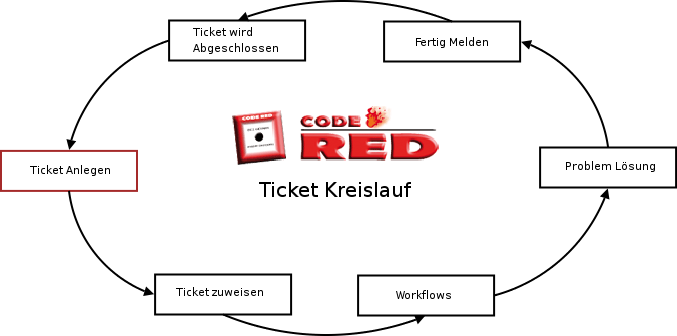
\includegraphics[width=450pt]{../bilder/Ticketkleislauf.png}
   \caption{Ticketkreislauf}
   \label{Ticketkreislauf}
\end{center}
\end{figure}
\vspace{2cm}
\begin{figure}[h]
\begin{center}
   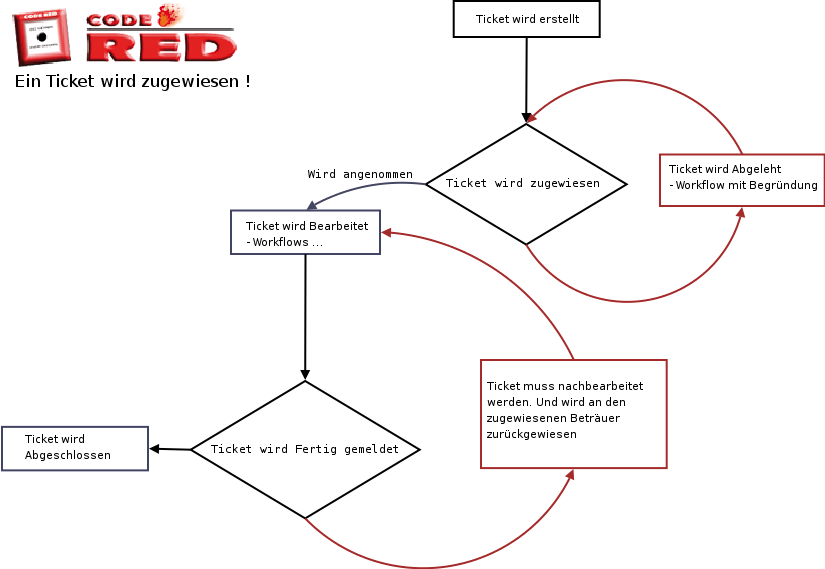
\includegraphics[width=450pt]{../bilder/Ticketzuweisung.png}
   \caption{Ticketzuweisung}
   \label{Ticketzuweisung}
\end{center}
\end{figure}

  
\chapter{Was sind Workflows?}  % Kapitel % Steht dann über dem Text
\label{chapter:Was sind Workflows?}  % Steht als Text im Inhaltsverzeichnis
\index{Was sind Workflows?} % für das Stichwortverzeichnis

Erklärung zu den Workflows?

urls bitte so:
\href{http://codered.berlios.de}{Codered Projektseite}


für consolen komandos:
\verb|kommando -option parameter|

\chapter{Personen Profile}  % Kapitel % Steht dann über dem Text
\label{chapter:Personen Profile}  % Steht als Text im Inhaltsverzeichnis
\index{Personen Profile} % für das Stichwortverzeichnis

Erklärung zu den Profilen

urls bitte so:
\href{http://codered.berlios.de}{Codered Projektseite}


für consolen komandos:
\verb|kommando -option parameter|



\part{CodeRed -Wer ist Wer?}
\label{part:Wer ist Wer?}
\chapter{Mentoren}  % Kapitel % Steht dann über dem Text
\label{chapter:Mentoren}  % Steht als Text im Inhaltsverzeichnis
\index{Mentoren} % für das Stichwortverzeichnis

Was sind und machen Mentoren

urls bitte so:
\href{http://codered.berlios.de}{Codered Projektseite}


für consolen komandos:
\verb|kommando -option parameter|

\input{clienten}
\chapter{Betreuer}  % Kapitel % Steht dann über dem Text
\label{chapter:Betreuer}  % Steht als Text im Inhaltsverzeichnis
\index{Betreuer} % für das Stichwortverzeichnis

\textbf{Die Betreuer},sind im Sinne des CodeRed Systems die Arbeiter. Betreuer sollen freiwillige Studierende der STSW werden. Grundsätzlich kann aber jedes Mitglied des Systems zu einem Betreuer hochgestuft werden.\\
Die Betreuer werden von den Mentoren beauftragt Tickets zu bearbeiten und zu dokumentieren. Sie selbst dürfen  keine Ticket zuweisen. Das Erstellen von Tickets ist ihnen aber möglich. \\
Sollte es vorkommen das ein Beteuer aus verschieden Gründen das Ticket nicht bearbeiten kann, darf er das ihm zugewiesene Ticket mit einer Erklärung zurückgeben. Ein Mentor kann dann das Ticket jemanden neu zuweisen. 
\\
\\
\textbf{Die Möglichkeiten von Betreuern im CodeRed System:}
\begin{figure}[h]
\begin{center}
   \includegraphics[width=400pt]{../bilder/betreuer.png}
   \caption{Systemstruktur- Betreuer}
   \label{Systemstruktur - Betreuer}
\end{center}
\end{figure}
\\
Der Betreuer hat die Pflicht das vom Mentoren zugewiesene Ticket, nach besten Wissen zu bearbeiten. Alle Arbeiten oder Gepräche über das Ticket sollen von Betreuer in Worksflows festgehalten werden. Sollte es ihm nicht möglich das Ticket zu bearbeiten, hat er jederzeit die Möglichkeit das Ticket zurückzugeben. Der Betreuer hat Zugriff auf alle Clienten und kann die vorhanden Dokumentationen der Clienten herunterladen oder/und auch eigene angefertigte Dokumentationen, zu dem jeweiligen Clienten, uploaden.


\chapter{Kontakte}  % Kapitel % Steht dann über dem Text
\label{chapter:Kontakte}  % Steht als Text im Inhaltsverzeichnis
\index{Kontakte} % für das Stichwortverzeichnis

Das System kennt drei verschiedene Usertypen die produktiv tätig sein können. Die Aufgaben und Möglichkeiten von Mentoren und Betreuer wurden schon auf den vorderen Seiten erklärt. \\
Die Kontakte sind die Personen, die als Ansprechpartner für die Clienten dienen. Von uns vorgesehen sind das Lehrer oder beauftragte von den verschieden Schulen die sich auch um die EDV Strukturen an den Schulen kümmern. \\
\\
\textbf{Aufgaben der Kontakte}\\
\begin{itemize}
\item Ansprechpartner für die Betreuer und Mentoren 
\item Kontakte verfassen hauptsächlich die Tickets für ihre Clienten
\item Pflege der Clienten  
\end{itemize}
 


\part{CodeRed -Future- u. Wishlist}
\label{part:Future- u. Wishlist}
\chapter{Bekannte Probleme!}  % Kapitel % Steht dann über dem Text
\label{chapter:Bekannte Probleme!}  % Steht als Text im Inhaltsverzeichnis
\index{Bekannte Probleme!} % für das Stichwortverzeichnis

\textbf{Warum läuft das System nur als Release Canidate 2?} \\
Leider konnte das nach unsere Meinung nach sehr wichtige E-Mail System in das CodeRed System nicht mehr rechtzeitig eingepflegt werden. Die Vorrausetzungen sind geschaffen und die Umsetzung sollte bis im Herbst dieses Jahres abgeschlossen sein. \\
\\
\textbf{Wie kann ich mein Passwort ändern?}\\
Leider ist das Ändern des User Passwortes in dieser Version der Software noch nicht möglich. Das Auslesen des verschlüsselten Passwortes und das dazugehörige Ändern des Passwortes konnte aus Zeitgründen im System nicht mehr verankert werden. 
Das Problem soll beim nächsten Update der Software behoben werden. \\
\\
\textbf{Erkennung von Dateitypen beim Upload von Dokumentationen}\\
Beim uploaden der Clienten Dokumentationen findet zur Zeit noch keine Dateitypen Erkennung statt. Diese Funktion war von uns angedacht konnte jedoch auch Zeitmangel nicht mehr implementiert werden. 

\chapter{Zukunftsmusik}  % Kapitel % Steht dann über dem Text
\label{chapter:Zukunftsmusik}  % Steht als Text im Inhaltsverzeichnis
\index{Zukunftsmusik} % für das Stichwortverzeichnis

Über die zukunft mit CodeRed und was wir dem System für ein potenzial zusprechen?
urls bitte so:
\href{http://codered.berlios.de}{Codered Projektseite}


für consolen komandos:
\verb|kommando -option parameter|




%Anhang
\backmatter
\appendix
\part{Anhang}
\label{part:Anhang}

%Entwurf von Tobias Mucke
%Erg�zungen von Michael Petter
%Kontext: SuSE 8.0
%Changelog:
%Timestamp                       Name                       �derungen und Begrndung
%26. Oktober 2002           Tobias Mucke        erweitert und korrigiert

\chapter{Literaturverzeichnis}
\begin{description}
\item{[1]}
Marco Benecke: \textit{Linux Installation, Konfiguration, Anwendung},
noch in planung :)

\end{description}






\printglossary

%Abbbildungsverzeichnis
\listoffigures

%Tabellenverzeichnis
\listoftables

%Listingverzeichnis
\lstlistoflistings

% Stichwortverzeichnis
\printindex

%Ende des Dokuments
\end{document}
